\documentclass{article}

\usepackage{hyperref}
\usepackage{fancyhdr}
\usepackage{braket}
\usepackage{extramarks}
\usepackage{amsmath}
\usepackage{amsthm}
\usepackage{amsfonts}
\usepackage{tikz}
\usepackage[plain]{algorithm}
\usepackage{algpseudocode}
\usepackage{mathtools}
\usepackage{graphicx}
\graphicspath{ {./Images/} }

\DeclarePairedDelimiter\abs{\lvert}{\rvert}%
\DeclarePairedDelimiter\norm{\lVert}{\rVert}%

\makeatletter
\let\oldabs\abs
\def\abs{\@ifstar{\oldabs}{\oldabs*}}
%
\let\oldnorm\norm
\def\norm{\@ifstar{\oldnorm}{\oldnorm*}}
\makeatother

\newcommand*{\Value}{\frac{1}{2}x^2}%

\usetikzlibrary{automata,positioning}

%
% Basic Document Settings
%

\topmargin=-0.45in
\evensidemargin=0in
\oddsidemargin=0in
\textwidth=6.5in
\textheight=9.0in
\headsep=0.25in

\linespread{1.1}

\pagestyle{fancy}
\lhead{\hmwkAuthorName}
\chead{\hmwkClass\ (\hmwkClassInstructor\ \hmwkClassTime): \hmwkTitle}
\rhead{\firstxmark}
\lfoot{\lastxmark}
\cfoot{\thepage}

\renewcommand\headrulewidth{0.4pt}
\renewcommand\footrulewidth{0.4pt}

\setlength\parindent{0pt}

%
% Create Problem Sections
%

\newcommand{\enterProblemHeader}[1]{
    \nobreak\extramarks{}{Problem \arabic{#1} continued on next page\ldots}\nobreak{}
    \nobreak\extramarks{Problem \arabic{#1} (continued)}{Problem \arabic{#1} continued on next page\ldots}\nobreak{}
}

\newcommand{\exitProblemHeader}[1]{
    \nobreak\extramarks{Problem \arabic{#1} (continued)}{Problem \arabic{#1} continued on next page\ldots}\nobreak{}
    \stepcounter{#1}
    \nobreak\extramarks{Problem \arabic{#1}}{}\nobreak{}
}

\setcounter{secnumdepth}{0}
\newcounter{partCounter}
\newcounter{homeworkProblemCounter}
\setcounter{homeworkProblemCounter}{1}
\nobreak\extramarks{Problem \arabic{homeworkProblemCounter}}{}\nobreak{}

%
% Homework Problem Environment
%
% This environment takes an optional argument. When given, it will adjust the
% problem counter. This is useful for when the problems given for your
% assignment aren't sequential. See the last 3 problems of this template for an
% example.
%
\newenvironment{homeworkProblem}[1][-1]{
    \ifnum#1>0
        \setcounter{homeworkProblemCounter}{#1}
    \fi
    \section{Problem \arabic{homeworkProblemCounter}}
    \setcounter{partCounter}{1}
    \enterProblemHeader{homeworkProblemCounter}
}{
    \exitProblemHeader{homeworkProblemCounter}
}

%
% Homework Details
%   - Title
%   - Due date
%   - Class
%   - Section/Time
%   - Instructor
%   - Author
%

\newcommand{\hmwkTitle}{Homework\ \#11}
\newcommand{\hmwkDueDate}{April 14, 2020}
\newcommand{\hmwkClass}{Physics 926}
\newcommand{\hmwkClassTime}{}
\newcommand{\hmwkClassInstructor}{Professor Ken Bloom}
\newcommand{\hmwkAuthorName}{\textbf{Robert Tabb}}

%
% Title Page
%

\title{
    \vspace{2in}
    \textmd{\textbf{\hmwkClass:\ \hmwkTitle}}\\
    \normalsize\vspace{0.1in}\small{Due\ on\ \hmwkDueDate\ at 5pm}\\
    \vspace{0.1in}\large{\textit{\hmwkClassInstructor\ \hmwkClassTime}}
    \vspace{3in}
}

\author{\hmwkAuthorName}
\date{}

\renewcommand{\part}[1]{\textbf{\large Part \Alph{partCounter}}\stepcounter{partCounter}\\}

%
% Various Helper Commands
%

% Useful for algorithms
\newcommand{\alg}[1]{\textsc{\bfseries \footnotesize #1}}

% For derivatives
\newcommand{\deriv}[1]{\frac{\mathrm{d}}{\mathrm{d}x} (#1)}

% For partial derivatives
\newcommand{\pderiv}[2]{\frac{\partial}{\partial #1} (#2)}

% Integral dx
\newcommand{\dx}{\mathrm{d}x}

% Alias for the Solution section header
\newcommand{\solution}{\textbf{\large Solution}}

% Probability commands: Expectation, Variance, Covariance, Bias
\newcommand{\E}{\mathrm{E}}
\newcommand{\Var}{\mathrm{Var}}
\newcommand{\Cov}{\mathrm{Cov}}
\newcommand{\Bias}{\mathrm{Bias}}

\begin{document}

\maketitle

\pagebreak

\begin{homeworkProblem}
	Show that
	\[
		P(\nu_1 \rightarrow \nu_2) = \sin^22\theta\sin^2\frac{\Delta m_{12}^2L}{4E}
	\]
	for a two neutrino system in which the mixing matrix is
	\[
		U=\begin{pmatrix}
		\cos\theta & \sin\theta \\
		-\sin\theta & \cos\theta
		\end{pmatrix}
	\]
	and $\Delta m_{12}^2=m_1^2-m_2^2$
	\\
	\\
	\textbf{Solution}
	\\
	\\
	Equation (7) from the lecture gives us a good starting point. This equation is an approximation which is valid when mass is small, which in this case it is
	\[
		P(\nu_1 \rightarrow \nu_2) = \abs{\sum_i U_{1i}^* U_{2i} e^{-im_i^2L/2E}}^2
	\]
	Using this equation as a starting point, we can plug in the given values of $U$ and explicitly do the sum.
	\[
		\begin{split}
		\abs{\sum_i U_{1i}^* U_{2i} e^{-im_i^2L/2E}}^2 =& \left[ \sum_i U_{1i}^* U_{2i} e^{-im_i^2L/2E} \right] \left[ \sum_j U_{1j}^* U_{2j} e^{-im_j^2L/2E} \right]^* \\
		=& \left[ \sum_i U_{1i}^* U_{2i} e^{-im_i^2L/2E} \right] \left[ \sum_j U_{2j}^* U_{1j} e^{im_j^2L/2E} \right] \\
		\sum_i U_{1i}^* U_{2i} e^{-im_i^2L/2E} =& \cos\theta(-\sin\theta) e^{-im_1^2L/2E} + \sin\theta\cos\theta e^{-im_2^2L/2E} \\
		=& -\cos\theta\sin\theta e^{-im_1^2L/2E} + \cos\theta\sin\theta e^{-im_2^2L/2E} \\
		=& \cos\theta\sin\theta \left( e^{-im_2^2L/2E} - e^{-im_1^2L/2E} \right) \\
		\sum_j U_{2j}^* U_{1j} e^{im_j^2L/2E} =& -\sin\theta\cos\theta e^{im_1^2L/2E} + \cos\theta\sin\theta e^{im_2^2L/2E} \\
		=& \cos\theta\sin\theta \left( e^{im_2^2L/2E} - e^{im_1^2L/2E} \right) \\
		\end{split}
	\]
	\[
		\begin{split}
		\left[ \sum_i U_{1i}^* U_{2i} e^{-im_i^2L/2E} \right] \left[ \sum_j U_{2j}^* U_{1j} e^{im_j^2L/2E} \right] =& \cos^2\theta\sin^2\theta \left( e^{-im_2^2L/2E} - e^{-im_1^2L/2E} \right) \left( e^{im_2^2L/2E} - e^{im_1^2L/2E} \right) \\
		=& \cos^2\theta\sin^2\theta \left( 2 - e^{i(m_1^2-m_2^2)L/2E} - e^{-i(m_1^2-m_2^2)L/2E} \right) \\		
		=& \cos^2\theta\sin^2\theta \left( 2 - 2Re\left[e^{i(m_1^2-m_2^2)L/2E}\right] \right) \\
		=& 2\cos^2\theta\sin^2\theta \left( 1 - \cos\frac{\Delta m_{12}^2L}{2E}  \right)
		\end{split}
	\]
	From here, use the trig identity: \(1-cos\theta = 2\sin^2\frac{\theta}{2}\) and then $2\cos\theta\sin\theta = \sin2\theta$:
	\[
		\begin{split}
		\left[ \sum_i U_{1i}^* U_{2i} e^{-im_i^2L/2E} \right] \left[ \sum_j U_{2j}^* U_{1j} e^{im_j^2L/2E} \right] =&  2\cos^2\theta\sin^2\theta \left( 2\sin^2\frac{\Delta m_{12}^2L}{4E}  \right) \\
		=& 4\cos^2\theta\sin^2\theta \left( \sin^2\frac{\Delta m_{12}^2L}{4E}  \right) \\
		=& \sin^22\theta \sin^2\frac{\Delta m_{12}^2L}{4E}
		\end{split}
	\]
	

\end{homeworkProblem}

\pagebreak

\begin{homeworkProblem}
	As an exercise in natural units, show that the quantity $\Delta m_{12}^2L/4E$ that appears in the theory of neutrino oscillations is in fact equal to $1.27\Delta m_{12}^2(eV^2)L(km)/E(GeV)$.
	\\
	\\
	\textbf{Solution}
	\\
	\\
	To start with, we know that the argument must be dimensionless since it is inside the sine function. And we see that in natural units we have \( [\Delta m_{12}^2][L]/[E] = GeV^2GeV^{-1}/GeV= \) dimensionless. Starting from these units, we can convert to $eV^2$ and $km$ to get the expression posed in the problem. In homework \#1, we had to derive conversion factors between natural units and SI units. In this problem we will use this to convert between length in $GeV^{-1}$ and $km$. The various ratios for conversions are:
	\[
		\begin{split}
		&L(GeV^{-1})=\frac{5.067\times 10^{15}\;GeV^{-1}}{1\;m}\frac{10^3 \; m}{1\; km}L(km) \\
		&\Delta m^2 (GeV^2) = \left( \frac{1\; GeV}{10^9\; eV} \right)^2 \Delta m^2 (eV^2)
		\end{split}
	\]
	Now plug these into the argument of the sine function from the previous problem to see what we get:
	\[
		\begin{split} 
		\frac{\Delta m^2 (GeV^2)L(GeV^{-1})}{4E(GeV)}=&\frac{\left( \frac{1\; GeV}{10^9\; eV} \right)^2 \Delta m^2 (eV^2)\frac{5.067\times 10^{15}\;GeV^{-1}}{1\;m}\frac{10^3 \; m}{1\; km}L(km)}{4E(GeV)} \\
		=& \frac{10^3}{10^{18}}\frac{5.067\times 10^{15}}{4}\frac{\Delta m^2 (eV^2)L(km)}{E (GeV)} \\
		=& 1.27 \frac{\Delta m^2 (eV^2)L(km)}{E (GeV)}
		\end{split}
	\]
\end{homeworkProblem}

\pagebreak

\begin{homeworkProblem}
	As mentioned in class, experiments such as NO$\nu$A are taking advantage of the fact that neutrinos that are traveling off-axis of a neutrino beam have a narrower energy spread. Let's take a look.
	\\
	\\
	(a) We want to make a neutrino beam from a beam of $\pi^+$ with $E_\pi = 20\; GeV$. How long should the decay pipe be to ensure the the great bulk of pions have decayed before they reach the absorber?
	\\
	\\
	(b) Consider a pion with energy $E_\pi$ in the laboratory frame. Find the energy of the neutrino $E_\nu$ in the decay $\pi^+\rightarrow \mu^+\nu_\mu$ as a function of the laboratory angle $\theta$ that the emitted neutrino makes with the original flight direction of the $\pi^+$.
	\\
	\\
	(c) Plot $E_\nu$ for $E_\pi$ between 2 and 20 $GeV$ in the case $\theta=0$ and $\theta=15 \; mrad$.
	\\
	\\
	\textbf{Solution}
	\\
	\\
	(a) Starting with the energy given, $E=20 \; GeV$, we can calculate velocity and time and use basic special relativity to get a good estimate. I am going to assume that the bulk of pions decaying means betwen 5 and 10 lifetimes (This may be a bit of an overestimate, but might as well err on the side of caution).
	\\
	\\
	Here are some relevant values:
	\[
		\begin{split}
		&\bar{\tau}=(2.603\pm 0.005)\times 10^{-8}s \\
		&m=0.14\; GeV = 1.78\times 10^{-27}\; kg \\
		&E=20\; GeV \\
		&p=\sqrt{E^2-m^2}\approx 20\;GeV = 1.07\times 10^{-17}\; kg\cdot m/s \\		
		\end{split}
	\]
	Where $\bar{\tau}$ is the mean lifetime, $m$ is the mass, $E$ is the energy, and $p$ is the momentum.\\
	Now I'll use these values to calculate velocity, lifetime in the rest frame of the particle, and thus the distance traveled.
	\[
		\begin{split}
		&p=\gamma mv=\frac{mv}{\sqrt{1-\frac{v^2}{c^2}}} \\
		&v=\frac{cp}{\sqrt{m^2c^2+\frac{p^2}{c^2}}} = \frac{(2.998\times 10^8)(1.07\times 10^{-17})}{\sqrt{(1.78\times 10^{-27}\cdot 2.998\times10^8)^2+\left(\frac{1.07\times 10^{-17}}{2.998\times 10^8}\right)^2}} \\
		&v=2.9979\times 10^8 m/s \approx 0.999976\; c \\
		&\gamma = \frac{1}{\sqrt{1-0.999976^2}} = 143.3 \\
		&\tau_{0,lower} = 5\gamma \bar{\tau} = 1.87\times 10^{-5}s \\
		&\tau_{0,upper} = 10\gamma \bar{\tau} = 3.73\times 10^{-5}s \\
		&d_{lower}=(2.9979\times 10^8)(1.87\times 10^{-5})  = 5.6\; km\\
		&d_{upper}=(2.9979\times 10^8)(3.73\times 10^{-5})  = 11.1\; km\\
		\end{split}
	\]
	Where $\tau_{0,lower}$ is the time estimate for five lifetimes, $\tau_{0,upper}$ is the time estimate for ten lifetimes, $d_{0,lower}$ is the distance using five lifetimes, and $d_{0,upper}$ is the distance using ten lifetimes. \\
	\\
	So based on my estimates the bulk of pions will be gone between $5.6$ and $11.1$ kilometers.
	\\
	\\
	(b) In the lab frame, the four-momenta of each particle can be defined. Let the initial direction of the pion be in the x-direction. ($\sigma$ is the index of the four-vectors while $\mu$ and $\nu$ are reserved for the muon and neutrino)
	\\
	\\
	Before the decay:
	\[
		P_\pi^\sigma = (E_\pi,p_\pi,0,0)
	\]
	After the decay:
	\[
		\begin{split}
		P_\mu^\sigma =& (E_\mu,\vec{p}_\mu) \\
		P_\nu^\sigma =& (E_\nu,p_\nu\cos\theta,p_\nu\sin\theta,0)
		\end{split}
	\]
	Note: I left the muon momentum completely general because it won't matter what value it has in the end.
	\\
	\\
	Due to conservation of four-momentum, we can write:
	\[
		\begin{split}
		P_\pi^\sigma = P_\mu^\sigma + P_\nu^\sigma \\
		P_\pi^\sigma - P_\nu^\sigma = P_\mu^\sigma \\		
		\end{split}
	\]
	We can contract each side with itself since this operation is Lorentz invariant:
	\[
		\begin{split}
		(P_\pi - P_\nu)^\sigma (P_\pi - P_\nu)_\sigma =& P_\mu^\sigma P_{\mu,\sigma} \\
		P_\pi^2+P_\nu^2-2P_\nu^\sigma P_{\pi,\sigma} =& P_\mu^2 \\
		m_\pi^2+m_\nu^2-2(E_\pi E_\nu-p_\pi p_\nu \cos\theta) =& m_\mu^2
		\end{split}
	\]
	$p_\nu \approx E_\nu$ because $m_\nu \approx 0$ compared with the other masses in the problem.
	\[
		\begin{split}		
		m_\pi^2-2(E_\pi E_\nu-m_\pi E_\nu \cos\theta) = m_\mu^2 \\
		m_\pi^2-m_\mu^2 = 2E_\nu(E_\pi-p_\pi \cos\theta) \\
		E_\nu = \frac{m_\pi^2-m_\mu^2}{2(E_\pi-p_\pi\cos\theta)} \\
		\end{split}
	\]
	But don't forget the dispersion relation:\(E^2=p^2+m^2\)
	\[
		\begin{split}
		\Rightarrow p_\pi = \sqrt{E_\pi^2-m_\pi^2}\\
		E_\nu = \frac{m_\pi^2-m_\mu^2}{2(E_\pi-\sqrt{E_\pi^2-m_\pi^2}\cos\theta)}
		\end{split}
	\]

	(c) Below is the plot of \(E_\nu = \frac{m_\pi^2-m_\mu^2}{2(E_\pi-\sqrt{E_\pi^2-m_\pi^2}\cos\theta)}\). 
	\begin{figure}[h]
		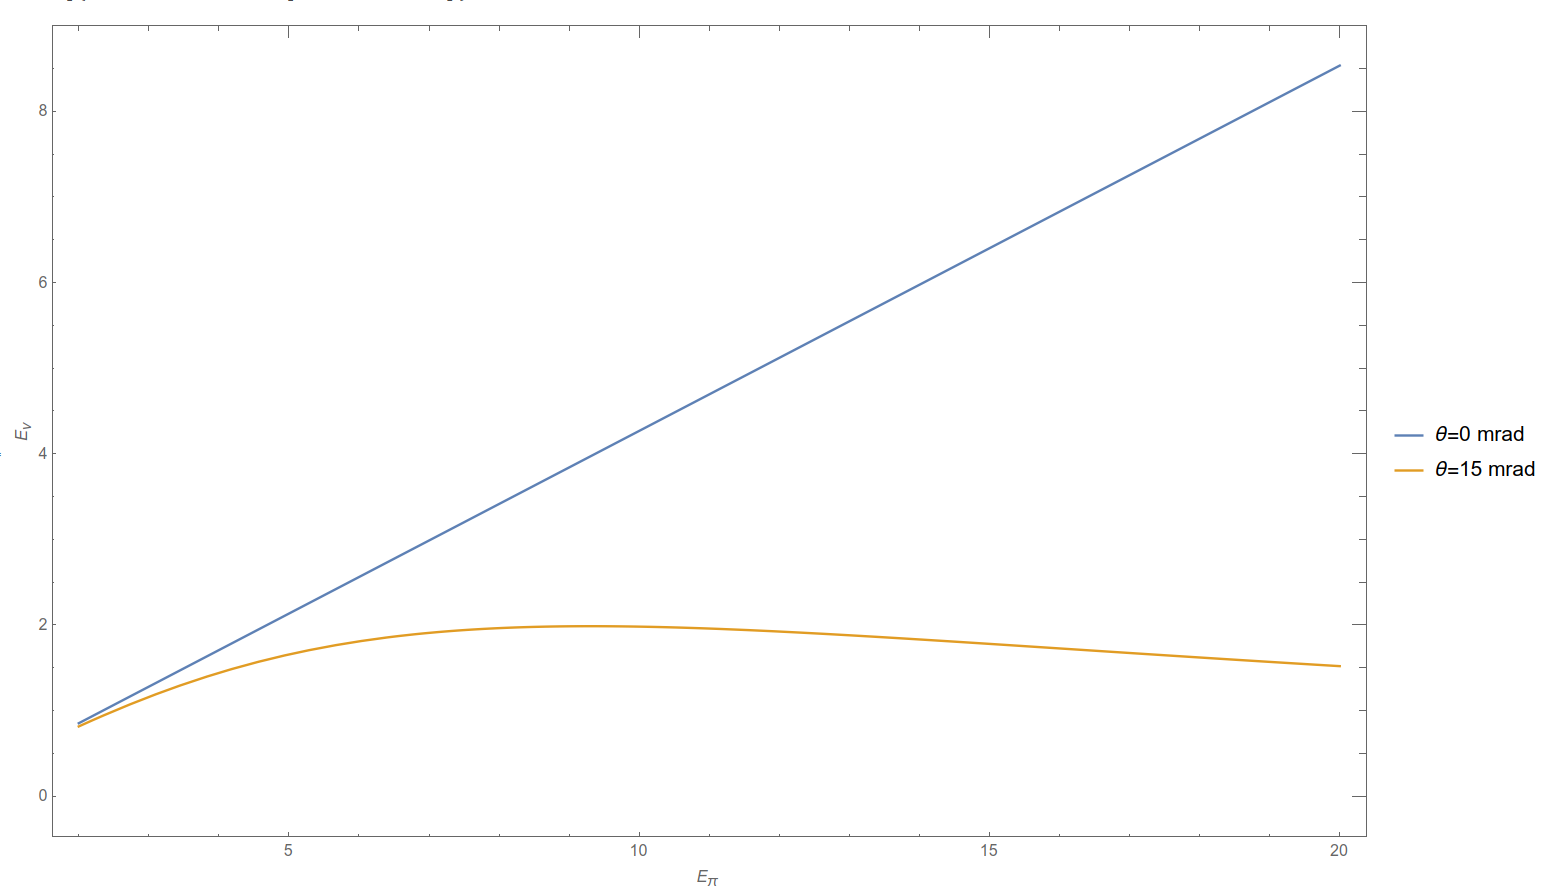
\includegraphics[scale=0.45]{prob3}
		\centering
		\caption{Neutrino energy as a function of pion energy for the decay, $\pi^+\rightarrow \nu_\mu \mu^+$}
		\label{prob3}
		\centering
	\end{figure}

\end{homeworkProblem}

\newpage

\begin{homeworkProblem} 
	We only briefly mentioned the possibility that neutrinos are their own antiparticles, i.e. are Majorana particles, and only briefly discussed the issue of CP violation. Let's explore these a little further. In class we said that for the three'generation mixing,
	\[
		P(\nu_\alpha \rightarrow \nu_\beta)= \delta_{\alpha\beta}-4\sum_{i>j}Re(U_{\alpha i}^*U_{\beta i}U_{\alpha j}U_{\beta j}^*)\sin^2\frac{\Delta m_{ij}^2L}{4E}+2\sum_{i>j}Im(U_{\alpha i}^*U_{\beta i}U_{\alpha j}U_{\beta j}^*)\sin\frac{\Delta m_{ij}^2L}{4E}
	\]
	Now, if neutrinos are Majorana particles, then the neutrino mixing matrix includes two extra Majorana phases, like so:
	\[
		U=\begin{pmatrix} 
		1 & 0 & 0\\
		0 & c_{23} & s_{23}\\
		0 & -s_{23} & c_{23}\end{pmatrix}
		\begin{pmatrix} 
		c_{13} & 0 & s_{13}e^{-i\delta} \\
		0 & 1 & 0 \\
		s_{13}e^{i\delta} & 0 & c_{13}\end{pmatrix}
		\begin{pmatrix} 
		c_{12} & s_{12} & 0 \\
		-s_{12} & c_{12} & 0 \\
		0 & 0 & 1\end{pmatrix}
		\begin{pmatrix} 
		e^{i\eta_1/2} & 0 & 0 \\
		0 & e^{i\eta_2/2} & 0 \\
		0 & 0 & 1\end{pmatrix}
	\]
	(a) Verify that these new phases have no effect on the oscillation probability.
	\\
	\\
	(b) As discussed in class, there is CP violation in neutrino oscillation if the imaginary term of the oscillation probability is non-zero for $\alpha \neq \beta$. Use the unitarity of the mixing matrix \(\left( \sum U_{\alpha i}U_{\beta i}^* =\delta_{\alpha\beta}\right) \) to show that for a given pair of flavors $\alpha$ and $\beta$ (with $\alpha\neq\beta$), the quantity $Im(U_{\alpha i}^*U_{\beta i}U_{\alpha j}U_{\beta j}^*)$ is the same (up to a sign) for any $i$ and $j$. This argument, based simply on unitarity, can be expanded by	interchanging the roles of the rows and columns of $U$ to conclude that for a given pair of $i$ and $j$ ($i \neq j$) the same quantity is independent of $\alpha$ and $\beta$ up to a sign. Thus, that quantity is universal, independent of $i$, $j$, $\alpha$ and $\beta$.
	\\
	\\
	(c) Use the expression for $U$ above, without the Majorana phases, to work out the value of the same imaginary quantity, with your favorite choice of $i$, $j$, $\alpha$, and $\beta$.
	(since it doesn’t matter what you choose). Verify that this quantity is proportional
	to $s_{12}s_{13}s_{23} \sin\delta$. This shows that CP violation needs not only a complex phase
	$\delta$ but also non-trivial mixing between all three neutrino states. If any of the
	rotation angles $\theta_{ij}$ is equal to $0$ or $\pi$, the CP violating effects disappear.
	\\
	\\
	\textbf{Solution}
	\\
	\\
	(a) To start, we'll multiply out the four matrices to get one matrix to refer to for each of the components of the probability equation. 
	\[
		\begin{split}
		U =& \begin{pmatrix} 
		c_{12}c_{13} & s_{12}c_{13} &  s_{13}e^{-i\delta} \\ 
		-s_{12}c_{23}-c_{12}s_{23}s_{13}e^{i\delta} & c_{12}c_{23}-s_{12}s_{23}s_{13}e^{i\delta} & s_{23}c_{13} \\
		s_{12}s_{23}-c_{12}c_{23}s_{13}e^{i\delta} & -c_{12}s_{23}-s_{12}c_{23}s_{13}e^{i\delta} & c_{23}c_{13}\\		
		\end{pmatrix}
		\begin{pmatrix} 
		e^{i\eta_1/2} & 0 & 0 \\
		0 & e^{i\eta_2/2} & 0 \\
		0 & 0 & 1\end{pmatrix} \\
		=& \begin{pmatrix} 
		c_{12}c_{13}e^{i\eta_1/2} & s_{12}c_{13}e^{i\eta_2/2} & s_{13}e^{-i\delta} \\
		-(s_{12}c_{23}+c_{12}s_{23}s_{13}e^{i\delta})e^{i\eta_1/2} & (c_{12}c_{23}-s_{12}s_{23}s_{13}e^{i\delta})e^{i\eta_2/2} & s_{23}c_{13} \\
		(s_{12}s_{23}-c_{12}c_{23}s_{13}e^{i\delta})e^{i\eta_1/2} & -(c_{12}s_{23}+s_{12}c_{23}s_{13}e^{i\delta})e^{i\eta_2/2} & c_{23}c_{13} 
		\end{pmatrix}
		\end{split}
	\]
	So let's use this to write out the parts of the probability equation that have the components of $U$ in it. 
	\[
		\begin{split}
		\sum_{i>j}(U_{\alpha i}^*U_{\beta i}U_{\alpha j}U_{\beta j}^*) =& -s_{12}c_{13}e^{-i\eta_2/2}(c_{12}c_{23}-s_{12}s_{23}s_{13}e^{i\delta})e^{i\eta_2/2}c_{12}c_{13}e^{i\eta_1/2}(s_{12}c_{23}+c_{12}s_{23}s_{13}e^{i\delta})e^{-i\eta_1/2} \\		
		=& -s_{12}c_{13}(c_{12}c_{23}-s_{12}s_{23}s_{13}e^{i\delta})c_{12}c_{13}(s_{12}c_{23}+c_{12}s_{23}s_{13}e^{i\delta})
		\end{split}
	\]
	As you can see, the additional phases all cancel each other out, so their addition to the matrix has no effect on the probability of oscillation.
	\\
	\\
	(b)
	\[
		\begin{split}
		\sum U_{\alpha i}U_{\beta i}^* =& U_{\alpha1}U_{\beta1}^*+U_{\alpha2}U_{\beta2}^*+U_{\alpha3}U_{\beta3}^* \\
		=& -c_{12}c_{13}(s_{12}c_{23}+c_{12}s_{23}s_{13}e^{-i\delta}) \\
		+& s_{12}c_{13}(c_{12}c_{23}-s_{12}s_{23}s_{13}e^{-i\delta}) \\
		+& s_{13}c_{23}c_{13}e^{-i\delta} \\
		=& -c_{12}c_{13}s_{12}c_{23}-c_{12}c_{13}c_{12}s_{23}s_{13}\cos\delta+ic_{12}c_{13}c_{12}s_{23}s_{13}\sin\delta \\
		+& s_{12}c_{13}c_{12}c_{23}-s_{12}c_{13}s_{12}s_{23}s_{13}\cos\delta+is_{12}c_{13}s_{12}s_{23}s_{13}\sin\delta \\
		+& s_{13}c_{23}c_{13}\cos\delta-is_{13}c_{23}c_{13}\sin\delta \\
		=& -(c_{12}c_{13}c_{12}s_{23}s_{13}+s_{12}c_{13}s_{12}s_{23})\cos\delta \\
		+&i(c_{12}c_{13}c_{12}s_{23}s_{13}+s_{12}c_{13}s_{12}s_{23}s_{13})\sin\delta \\
		\Rightarrow & i(c_{12}c_{13}c_{12}s_{23}s_{13}+s_{12}c_{13}s_{12}s_{23}s_{13})\sin\delta = (c_{12}c_{13}c_{12}s_{23}s_{13}+s_{12}c_{13}s_{12}s_{23})\cos\delta \\
		\Rightarrow & \tan\delta = -i
		\end{split}
	\]

	(c)
	\[
		\begin{split}
		Im(U_{1,1}^*U_{2,1}U_{1,3}U_{2,3}^*) =& Im[-c_{12}c_{13}(s_{12}c_{23}+c_{12}s_{23}s_{13}e^{i\delta})s_{13}s_{23}c_{13}e^{-i\delta}] \\
		=& Im[-c_{12}c_{13}s_{12}c_{23}s_{13}s_{23}c_{13}e^{-i\delta}-c_{12}c_{13}c_{12}s_{23}s_{13}s_{13}s_{23}c_{13}] \\
		=& c_{12}c_{13}s_{12}c_{23}s_{13}s_{23}c_{13}\sin\delta
		\end{split}
	\] 
	\[
	\begin{split}
	Im(U_{1,2}^*U_{3,2}U_{1,3}U_{3,3}^*) =& -s_{12}c_{13}(c_{12}s_{23}+s_{12}c_{23}s_{13}e^{i\delta})s_{13}c_{23}c_{13}e^{-i\delta} \\
	=& Im[-s_{12}c_{13}c_{12}s_{23}s_{13}c_{23}c_{13}e^{-i\delta}-s_{12}c_{13}s_{12}c_{23}s_{13}s_{13}c_{23}c_{13}] \\
	=& s_{12}c_{13}c_{12}s_{23}s_{13}c_{23}c_{13}\sin\delta
	\end{split}
	\] 
	I got the same value for two different arbitrarily chosen indices, but the factors in front of the $\sin\delta$ are not the same as those in the problem. I am unsure where I have gone wrong.
\end{homeworkProblem}
\end{document}

